\documentclass[a4paper,12pt]{report}
\usepackage[utf8]{inputenc}
\usepackage[italian]{babel}
\usepackage[hidelinks]{hyperref}
\usepackage{graphicx}
\usepackage{lmodern}
\usepackage{setspace}
\usepackage{geometry}
\usepackage{titlesec}
\usepackage{fancyhdr}
\usepackage{tocloft}
\usepackage{etoolbox}
\geometry{margin=2cm}

% Numerazione sezioni e sottosezioni
\renewcommand{\thesection}{\thechapter.\arabic{section}}
\renewcommand{\thesubsection}{\thesection.\arabic{subsection}}
\setcounter{secnumdepth}{2}
\setcounter{tocdepth}{2}

% Font per sezioni
\titleformat{\section}
  {\normalfont\small\bfseries}
  {\thesection}{1em}{}

\titleformat{\subsection}
  {\normalfont\small\itshape}
  {\thesubsection}{1em}{}



%impostazione personalizzate per linee di codice
\usepackage{listings}
\usepackage[x11names]{xcolor}
\definecolor{MyGreen}{HTML}{16610E}

\lstset{
  basicstyle=\ttfamily\footnotesize,
  breaklines=true,
  breakatwhitespace=true,
  keywordstyle=\color{blue},
  commentstyle=\color{gray},
  stringstyle=\color{MyGreen},
  showstringspaces=false,
  columns=fullflexible,
  language=Python
}

% Impostazioni personalizzate per capitoli e piè di pagina
\titleformat{\chapter}[block]
  {\normalfont\Huge\bfseries}
  {\relax} % rimuove "Capitolo N"
  {0pt}
  {}

\pagestyle{fancy}
\fancyhf{}
\fancyfoot[C]{Capitolo \thechapter\ -- \thepage}


\begin{document}

% --- Copertina ---
\begin{titlepage}
    \begin{center}
        
\includegraphics[width=0.4\textwidth]{logo-universita.png}
        \Large\textbf{UNIVERSIT\`A DEGLI STUDI DI CATANIA}\\[0.3cm]
        \large Dipartimento di Matematica e Informatica\\
        \large Corso di Laurea Triennale in Informatica\\[2cm]

        \vspace{2cm}

        {\Huge \textbf{VolleyLive}}\\[0.5cm]
        {\large Sistema di monitoraggio, analisi e visualizzazione\\
        delle partite di pallavolo in tempo reale}\\[2.5cm]

        \vspace{1cm}

        \begin{flushleft}
            \textbf{Studente:} \\
            Claudio Nuncibello
        \end{flushleft}

        \vspace{1cm}

        \begin{flushright}
            \textbf{Relatore:} \\
            Prof. Salvatore Nicotra
        \end{flushright}

        \vfill

        \textbf{Anno Accademico 2024/2025}
    \end{center}
\end{titlepage}

% --- Abstract e logo ---
\newpage
\thispagestyle{empty}
\vspace*{2cm}
\begin{center}
    
\includegraphics[width=0.4\textwidth]{volleylive-logo.png} \\[1.5cm]
    \textbf{\LARGE Abstract} \\[1cm]
    \begin{minipage}{0.85\textwidth}
        \small
        Il progetto VolleyLive nasce con l’obiettivo di monitorare e analizzare in tempo reale le partite di pallavolo, combinando tecnologie moderne per la gestione dei dati in streaming e la visualizzazione interattiva. Il sistema raccoglie snapshot live da API sportive, li trasforma e li distribuisce tramite una pipeline composta da Kafka, Logstash, Spark ed Elasticsearch. I dati vengono visualizzati in una dashboard frontend sviluppata in Next.js, offrendo funzionalit\`a come la selezione dei match preferiti e l’analisi predittiva dell’esito delle partite. L’intero progetto \`e containerizzato tramite Docker e supporta l’estensibilit\`a verso nuovi modelli e sport. Questa tesi descrive l’architettura, le scelte progettuali, e i risultati ottenuti attraverso l’implementazione del sistema.
    \end{minipage}
\end{center}
\newpage

% --- Indice ---
\tableofcontents
\newpage

% ===============================
% INTRODUZIONE
% ===============================
\chapter*{Introduzione}
\addtocontents{toc}{\vspace{0.3cm}\textbf{Introduzione}\par}

Il presente elaborato descrive lo sviluppo di VolleyLive: un sistema per il monitoraggio e l’analisi in tempo reale delle partite di pallavolo. Il progetto nasce nell’ambito dell’analisi sportiva, oggi profonda trasformazione, favorita dalla crescente disponibilità di dati e dall’utilizzo di tecnologie per l’elaborazione in streaming. L’integrazione di API sportive, strumenti di monitoraggio e algoritmi analitici consente oggi non solo di osservare lo svolgimento di una competizione, ma anche di interpretarne dinamicamente l’andamento e prevederne l’evoluzione. L’analisi in tempo reale ha assunto un ruolo centrale in numerosi ambiti applicativi, dallo sport professionale alla logistica industriale. Nel mondo sportivo tuttavia strumenti avanzati di elaborazione live sono spesso riservati a discipline molto seguite (come calcio o basket), o a contesti professionali ad alto budget. Per molte altre discipline come la pallavolo esistono margini significativi per migliorare l’accessibilità e la fruibilità dei dati durante gli eventi. VolleyLive non si propone soltanto come una soluzione funzionale per il monitoraggio in tempo reale, ma getta le basi per un sistema estensibile e orientato al futuro delle competizioni sportive. Grazie all’adozione di tecnologie scalabili e open source, la piattaforma si presta a essere ampliata per integrare nuove fonti dati e modelli predittivi sempre più sofisticati. In questo senso, VolleyLive rappresenta una prima esplorazione concreta verso sistemi intelligenti di supporto all’analisi sportiva, potenzialmente applicabili non solo alla pallavolo ma a molte altre discipline. Il sistema adotta tecnologie all'avanguardia come Kafka per la gestione del flusso dati, Logstash per la trasformazione degli eventi, Spark per l’elaborazione in tempo reale, Elasticsearch per l’indicizzazione e la consultazione, e una web app per la visualizzazione lato utente. Il tutto è orchestrato tramite container Docker, in modo da garantire portabilità, isolamento e semplicità di gestione. Gli obiettivi principali del progetto sono: costruire una pipeline dati solida e scalabile, in grado di gestire flussi continui di snapshot aggiornati ogni dieci secondi; applicare modelli di analisi per stimare in tempo reale l’esito delle partite in corso; offrire un’interfaccia intuitiva e interattiva per la consultazione live dei match; garantire la tracciabilità storica dei dati raccolti, utile per analisi retrospettive e sviluppo futuro di modelli predittivi più avanzati. Dal punto di vista applicativo, VolleyLive è pensato per essere utilizzato sia da utenti generici interessati a seguire una competizione sia da figure più tecniche come data analyst sportivi o scout, che necessitano di uno strumento semplice ma flessibile per leggere, filtrare e confrontare partite in tempo reale. L'elaborato è articolata in sette capitoli. Nel capitolo primo capitolo si descriverà l’architettura generale del sistema e i componenti principali, soffermandosi sulle tecnologie adottate e sul loro ruolo nella pipeline. Il secondo capitolo approfondirà il funzionamento della raccolta dati live tramite API e il terzo illustra i meccanismi di ingestione, trasformazione ed elaborazione in streaming. Il quarto capitolo è dedicato alla visualizzazione e all’interazione tramite dashboard web. Il quinto capitolo presenta una serie di risultati ottenuti attraverso l’esecuzione del sistema, evidenziando esempi pratici e scenari d’uso. nelle conclusioni si raccolgono le riflessioni conclusive e suggerisce direzioni per futuri sviluppi ed estensioni. VolleyLive si propone quindi come una base concreta per sperimentare tecnologie moderne per lo streaming e l’analisi dei dati sportivi, ponendo particolare attenzione all’affidabilità del flusso, alla chiarezza della visualizzazione e alla possibilità di estensione verso altri sport o contesti analitici.

% ===============================
% CAPITOLO 1 - Architettura
% ===============================

\chapter{Architettura Generale del Sistema}

Il sistema VolleyLive è stato concepito e realizzato seguendo un approccio modulare e scalabile, con l’obiettivo di garantire affidabilità, continuità del flusso dati e facilità di estensione. Questo capitolo descrive nel dettaglio l’architettura generale adottata, soffermandosi su ciascuna delle tecnologie impiegate, sul ruolo che ricoprono nella pipeline e sulle relazioni tra i vari moduli.


\section{Panoramica dei Componenti Tecnologici}

In questa sezione si fornisce una descrizione dettagliata dei principali componenti tecnologici che costituiscono il sistema VolleyLive, evidenziando il ruolo operativo di ciascun modulo all’interno della pipeline. Ogni tecnologia è presentata nel contesto del suo impiego pratico, illustrandone le funzionalità chiave e le modalità con cui interagisce con gli altri elementi del sistema.


\subsection{Fonte Dati: SportDevs API}

Il sistema VolleyLive si basa sui dati forniti dalle API pubbliche di SportDevs, che rappresentano la fonte principale per l’acquisizione delle informazioni relative alle partite in corso. Queste API espongono una serie di endpoint REST, interrogabili in formato \texttt{JSON}, attraverso cui è possibile ottenere dati grezzi aggiornati sulle partite live, dai quali il sistema costruisce, tramite successive trasformazioni, snapshot strutturati e coerenti, idonei a essere impiegati nei modelli di previsione.

Nel flusso di sistema, le API costituiscono il punto iniziale della pipeline: i dati vengono estratti regolarmente dallo script \textit{producer}, che li interroga ogni dieci secondi. I dati ricevuti vengono normalizzati e strutturati per essere inoltrati a Kafka nel formato previsto. L'accesso avviene tramite chiave API e richiede attenzione nella gestione della frequenza di interrogazione per evitare di superare i limiti imposti dal servizio.

Nonostante l’ampia copertura e il buon livello di dettaglio, le API presentano alcune limitazioni. In particolare, durante le partite di campionati minori si riscontrano occasionali ritardi nell’aggiornamento dei punteggi, e la gestione del set di \textit{tiebreak} può risultare imprecisa o mancante. Queste problematiche sono note e, al momento, vengono gestite a livello applicativo convivendo con le possibili incongruenze nel dato.

Nel complesso, SportDevs rappresenta una soluzione efficace per alimentare in tempo reale il sistema VolleyLive, pur richiedendo l’adozione di logiche resilienti in fase di raccolta e validazione dei dati.

\subsection{Elaborazione e Normalizzazione: Logstash}

Logstash è il primo componente della pipeline incaricato della trasformazione dei dati in arrivo dalle API di VolleyLive. Riceve direttamente i dati grezzi forniti dallo script Python (producer), li interpreta e li converte in un formato strutturato, adatto alla successiva pubblicazione su Kafka.

Le operazioni svolte da Logstash includono la normalizzazione dei nomi dei campi, l’estrazione di \textit{timestamp} coerenti, la gestione di dati opzionali o incoerenti, e l’aggiunta di metadati utili (come gli identificativi univoci del match). Queste trasformazioni avvengono tramite pipeline configurabili in formato dichiarativo, che permettono di adattare con facilità le regole di parsing e filtraggio.

Una volta completata l’elaborazione, Logstash pubblica gli \textit{snapshot} trasformati su un \textit{topic} Kafka, rendendoli disponibili per le successive fasi di analisi e indicizzazione. In questo modo, Logstash funge da punto di ingresso intelligente per il flusso dati del sistema, garantendo uniformità e qualità nella base informativa di VolleyLive.


\subsection{Gestione del Flusso Dati: Kafka}

Apache Kafka è il sistema di messaggistica distribuito adottato da VolleyLive per la gestione affidabile e scalabile del flusso dati in tempo reale. All’interno dell’architettura, Kafka riceve i dati già trasformati da Logstash e li rende disponibili per i successivi moduli di analisi e indicizzazione.

Ogni snapshot elaborato viene pubblicato su un \textit{topic} Kafka, da cui può essere consumato in parallelo da più servizi, come Apache Spark o eventuali altri moduli analitici. Questo modello basato su pubblicazione e sottoscrizione (\textit{pub/sub}) consente un’elaborazione asincrona, modulare e facilmente estendibile.

La scelta di utilizzare Kafka è stata motivata dalla necessità di gestire un flusso continuo di eventi con frequenti aggiornamenti, mantenendo elevate garanzie di durabilità, ordinamento e possibilità di \textit{replay} dei messaggi. La sua architettura nativamente distribuita lo rende particolarmente adatto a scenari \textit{real-time} come quello di VolleyLive.


\subsection{Analisi Streaming: Apache Spark}

Apache Spark è il componente dedicato all’elaborazione avanzata dei dati in streaming nel sistema VolleyLive. Dopo che gli \textit{snapshot} sono stati pubblicati su Kafka da Logstash, Spark li consuma in tempo reale per applicare logiche analitiche e generare output destinati all’indicizzazione.

L’implementazione sfrutta Spark Structured Streaming, un sistema che elabora i dati in tempo reale suddividendoli in piccoli blocchi temporali (\textit{micro-batch}). Anche se i dati arrivano in modo continuo, Spark li raggruppa ogni pochi secondi e li processa in modo ordinato e affidabile. Questo approccio garantisce una \textit{semantica end-to-end}, ovvero l’elaborazione completa, senza perdite o duplicazioni, di ogni blocco di dati dall’ingresso all’output finale.

Nel contesto di VolleyLive, Spark viene utilizzato per applicare filtri, trasformazioni strutturali e, in prospettiva, funzioni di analisi predittiva basate su modelli di \textit{machine learning}.

Spark si colloca tra la distribuzione dei dati (Kafka) e la fase di visualizzazione (Elasticsearch), fungendo da nodo di elaborazione intermedio. Questa configurazione permette di isolare la logica analitica dal resto della pipeline, semplificando l’estensione futura del sistema verso algoritmi più sofisticati.


\subsection{Indicizzazione e Ricerca: Elasticsearch}

Elasticsearch è il motore di ricerca e indicizzazione adottato nel sistema VolleyLive per rendere interrogabili e visualizzabili gli \textit{snapshot} elaborati in tempo reale. Dopo l’elaborazione su Apache Spark, ogni snapshot viene inviato a Elasticsearch, dove viene memorizzato come documento JSON strutturato.

Tutti i dati, inclusi gli score predittivi e le informazioni live, vengono inseriti all’interno di un unico indice. Questa scelta progettuale consente di ottenere, tramite una singola query, tutte le informazioni aggiornate relative a un match, semplificando l’accesso lato frontend e migliorando l’efficienza delle chiamate.

L’indice è configurato con un \textit{mapping} coerente, che definisce esplicitamente la struttura e i tipi dei campi per garantire interrogazioni affidabili e prestazioni ottimali. Questo approccio assicura una base dati consistente e facilmente estendibile anche in fase di evoluzione del sistema.

Infine, per attività di \textit{debugging}, monitoraggio e ispezione manuale dei dati, il sistema fa uso di Kibana, uno strumento di visualizzazione integrato con Elasticsearch, utile in particolare durante le fasi di sviluppo.


\subsection{Visualizzazione: Frontend React/Next.js}

L’interfaccia utente di VolleyLive è sviluppata utilizzando il framework React in combinazione con Next.js, una soluzione moderna e performante per la realizzazione di applicazioni web dinamiche. Il frontend fornisce agli utenti una dashboard interattiva e reattiva per consultare lo stato in tempo reale delle partite, visualizzare punteggi, set e score predittivi.

Per accedere ai dati, il frontend comunica con un backend intermedio realizzato in FastAPI. Questo backend funge da strato di accesso alle informazioni archiviate in Elasticsearch, esponendo API REST personalizzate per effettuare query sui match live. Tale approccio consente di mantenere il database isolato, migliorare la sicurezza e semplificare la gestione delle richieste dal lato client.

La struttura della dashboard permette agli utenti di selezionare match preferiti live e visualizzare in dettaglio l’andamento di ciascun incontro. L’interfaccia è stata progettata per adattarsi ai diversi dispositivi.

Il frontend è containerizzato e integrato nell’infrastruttura tramite Docker, in modo da garantire coerenza tra ambiente di sviluppo e produzione e facilitare il deployment del sistema completo.


\subsection{Containerizzazione: Docker e Visualizzazione dell’Architettura}

Il sistema VolleyLive adotta una configurazione interamente containerizzata, implementata tramite Docker, al fine di garantire portabilità, isolamento e semplicità di gestione in tutte le fasi del ciclo di vita dell’applicazione. Ogni componente è incapsulato in un container indipendente, facilitando la manutenzione, il testing e il deployment multiambiente.

L’infrastruttura è orchestrata mediante \texttt{docker-compose}, che consente di avviare l’intero ecosistema tramite un’unica configurazione centralizzata. I servizi comunicano all’interno di una rete virtuale definita da Docker, riducendo le dipendenze esterne e i problemi di configurazione ambientale.

Tutti i moduli descritti nei paragrafi precedenti – inclusi il \textit{producer} Python, i servizi di elaborazione e analisi, l’API backend e l’interfaccia web – sono containerizzati e integrati nell’infrastruttura, assicurando coerenza tra ambiente di sviluppo e produzione.

Lo schema architetturale riportato in Figura~\ref{fig:architettura} illustra il flusso dei dati e le interazioni principali tra i servizi, dalla raccolta degli snapshot fino alla visualizzazione finale.

\begin{figure}[ht]
    \centering
    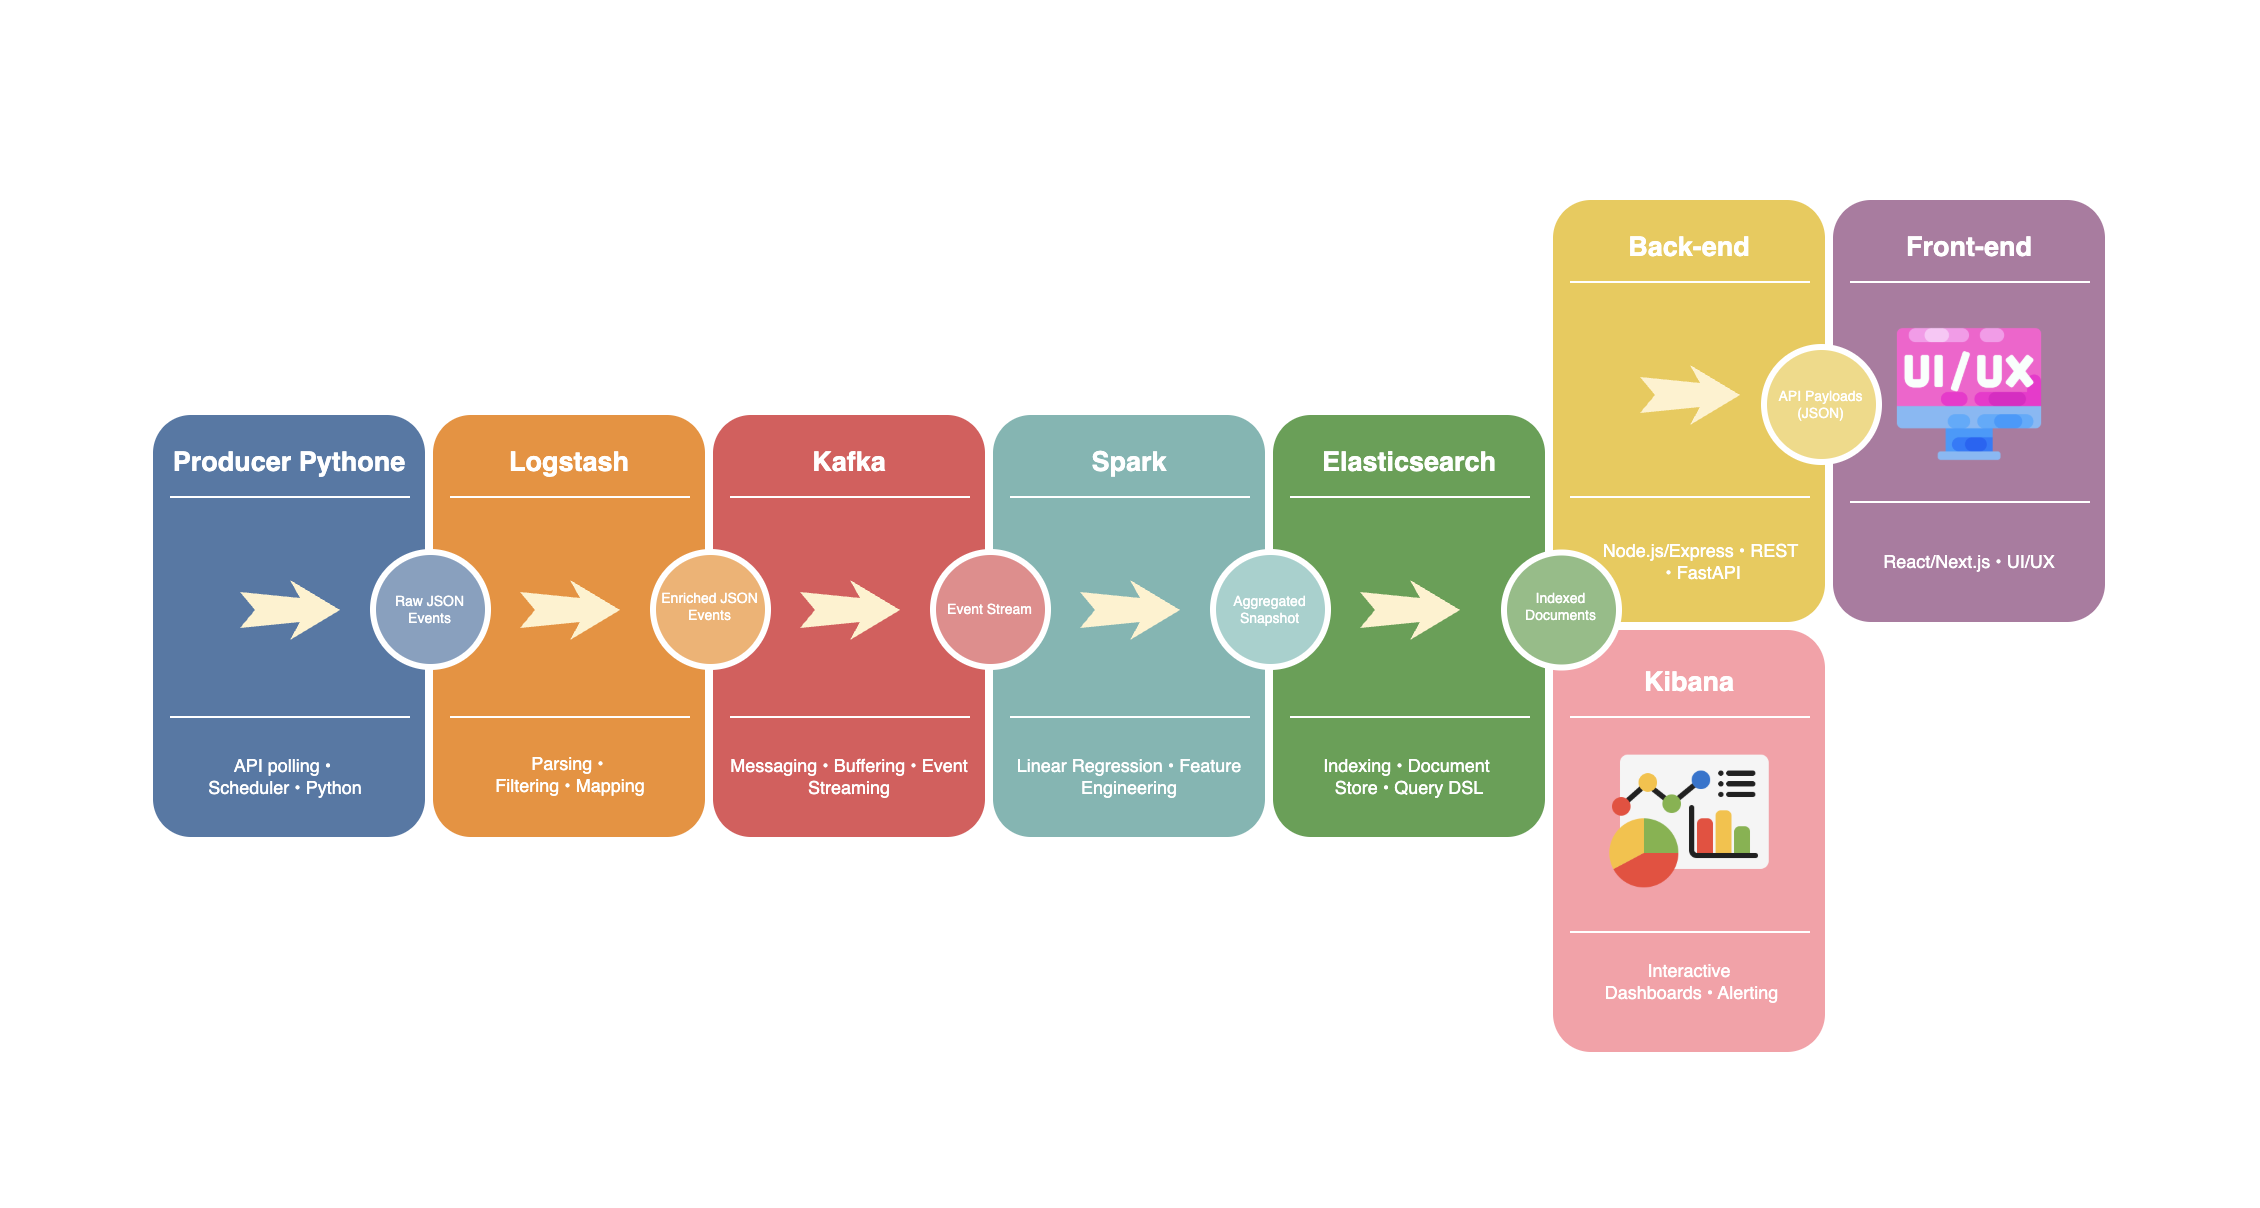
\includegraphics[width=0.9\textwidth]{schema-architettura.png}
    \caption{Architettura containerizzata del sistema VolleyLive}
    \label{fig:architettura}
\end{figure}


\section{Scelte Progettuali e Motivazioni}

La definizione dell’architettura di VolleyLive è frutto di un processo decisionale che ha bilanciato esigenze di efficienza, semplicità operativa e finalità analitiche.
In questa sezione vengono descritte le principali alternative valutate e le motivazioni che hanno portato alla definizione dell’architettura presentata nel paragrafo precedente.

\subsection{Pipeline Always-On vs On-Demand: Analisi Comparativa}

Nel progettare il sistema VolleyLive, si è valutata la possibilità di attivare la pipeline dati solo in risposta a un’azione dell’utente (approccio \textit{on-demand}) oppure di mantenerla costantemente attiva (approccio \textit{always-on}). La modalità \textit{on-demand}, sebbene più leggera dal punto di vista computazionale, avrebbe comportato una latenza iniziale, una complessità maggiore nel coordinamento tra moduli e una perdita della continuità storica. L’approccio \textit{always-on} garantisce invece un flusso costante e affidabile di dati, semplificando il design complessivo e consentendo l’elaborazione in tempo reale anche in assenza di richieste attive.

\subsection{Motivazioni della Scelta dell’Architettura Always-On}

L’adozione dell’architettura \textit{always-on} è stata guidata da due esigenze fondamentali: da un lato, garantire l’affidabilità e la continuità del flusso dati; dall’altro, costruire una base dati storica che consenta analisi retrospettive e l’applicazione di modelli predittivi. Inoltre, la natura del progetto – focalizzato sull’utilizzo di tecnologie di data streaming e containerizzazione – trova piena espressione in un sistema sempre attivo, che riflette in modo coerente gli obiettivi sperimentali della tesi.


% ===============================
% CAPITOLO 2 - Pipeline dei Dati Live
% ===============================

\chapter{Acquisizione e Gestione dei Dati in Real-Time}

In questo capitolo viene descritta la prima parte della pipeline utilizzata da VolleyLive, dedicata alla raccolta e alla gestione iniziale dei dati provenienti da partite di pallavolo in corso. Il focus sarà sulle tecnologie e le metodologie impiegate per acquisire dati live, trasformarli in un formato standardizzato e distribuirli attraverso un flusso dati affidabile e scalabile.

I paragrafi di questo capitolo affrontano in maniera approfondita ciascuno dei passaggi fondamentali: dall'acquisizione iniziale tramite script Python, alla normalizzazione effettuata da Logstash, fino alla distribuzione tramite Kafka. Ogni fase sarà illustrata nel dettaglio, sottolineando le scelte tecniche effettuate e le loro motivazioni.

\section{Acquisizione Dati: Producer Python}

\subsection{Introduzione agli Snapshot Live}

Nella pipeline dati del progetto VolleyLive, lo snapshot live rappresenta il punto iniziale e fondamentale per ogni successiva elaborazione ed analisi. Per snapshot si intende una fotografia periodica e dettagliata dello stato corrente di ciascuna partita monitorata. Tali istantanee sono catturate a intervalli temporali regolari (ogni pochi secondi), al fine di garantire una visione costantemente aggiornata degli eventi sportivi in corso.

L’impiego degli snapshot live si rivela cruciale poiché essi costituiscono non solo la base per l’analisi in tempo reale, ma anche una risorsa fondamentale per alimentare il dataset storico, contribuendo così a migliorare nel tempo l’accuratezza delle predizioni effettuate dal sistema.


\subsection{API SportDevs: Dati e Endpoint Utilizzati}

La raccolta dei dati live viene effettuata interrogando direttamente le API pubbliche di SportDevs, che permettono di accedere a informazioni aggiornate in tempo reale sulle partite di pallavolo. Queste API restituiscono dati in formato JSON, facilmente integrabili all'interno del sistema VolleyLive.
Il producer Python utilizza principalmente tre endpoint. Il primo è:

\url{https://volleyball.sportdevs.com/matches?status_type=eq.live}

Questo endpoint restituisce tutte le partite attualmente in corso e fornisce i dati essenziali per comporre uno snapshot live, come il punteggio per ciascun set, lo stato della partita, gli ID delle squadre coinvolte e altre informazioni contestuali.
Il secondo endpoint utilizzato è:

\url{https://volleyball.sportdevs.com/matches?or=(home_team_id.eq.{team_id},away_team_id.eq.{team_id})&order=specific_start_time.desc&limit=5}

Questo viene impiegato per ottenere gli ultimi cinque incontri disputati da una specifica squadra, identificata dal parametro \texttt{team\_id}. Tali informazioni possono essere utilizzate per arricchire gli snapshot con contesto storico immediato.
Infine, il terzo endpoint è:

\url{https://volleyball.sportdevs.com/matches?or=(and(home_team_id.eq.{home_id},away_team_id.eq.{away_id}),and(home_team_id.eq.{away_id},away_team_id.eq.{home_id}))&order=specific_start_time.desc&limit=20}

Questo permette di recuperare lo storico degli scontri diretti (head-to-head) tra due squadre, fornendo un quadro comparativo utile tra avversarie ricorrenti.

Le richieste a questi endpoint vengono eseguite periodicamente, con gestione dei token di autenticazione quando necessario. I dati ottenuti vengono poi pre-processati dal producer per adattarli al formato previsto dalla pipeline.

\subsection{Trasformazioni e Feature Addizionali}

A valle della raccolta dei dati grezzi dagli endpoint SportDevs, lo script Python applica un processo di trasformazione che arricchisce ogni snapshot con una serie di colonne derivate, necessarie per semplificare l’analisi nei passaggi successivi e per arricchire la semantica delle informazioni trasmesse.
Vengono innanzitutto calcolati i punteggi totali aggiornati per ciascuna squadra (\texttt{home\_score\_total} e \texttt{away\_score\_total}) e la loro differenza (\texttt{score\_diff}), utile per valutare rapidamente l’andamento della partita. A questi si aggiunge la differenza tra il numero di set vinti dalle due squadre, rappresentata nella colonna \texttt{set\_diff}. Lo stato del set in corso viene descritto tramite i punteggi parziali (\texttt{home\_current\_score} e \texttt{away\_current\_score}) e una rappresentazione sintetica della situazione (\texttt{set\_info}), come ad esempio ``Set 3: 18--22''.
L’arricchimento dello snapshot prosegue con l’inserimento di tre metriche derivate da partite storiche: \texttt{home\_win\_rate\_last5} e \texttt{away\_win\_rate\_last5} indicano le percentuali di vittorie delle due squadre negli ultimi cinque match disputati, mentre \texttt{head\_to\_head\_win\_rate\_home} riflette il tasso di vittorie della squadra di casa negli scontri diretti più recenti contro l’avversaria.

Per quanto riguarda i dati storici, che richiederebbero interrogazioni multiple verso gli endpoint /matches. Per ottimizzare le prestazioni e ridurre la frequenza di chiamate HTTP, viene implementato un sistema di caching locale: quando le partite storiche di una determinata squadra o di una coppia di squadre sono già state scaricate in una precedente iterazione, i dati vengono riutilizzati evitando ulteriori richieste. Questo approccio consente di mantenere l’aggiornamento in tempo reale senza sovraccaricare l’infrastruttura remota.

Tutte le trasformazioni vengono applicate prima dell’invio dello snapshot a Logstash, contribuendo a mantenere leggerezza e modularità nelle componenti a valle della pipeline, che possono così concentrarsi sull’analisi e sull’indicizzazione dei dati già strutturati.

\section{Elaborazione e Normalizzazione: Logstash}

Una volta generati dal producer Python, gli snapshot arricchiti vengono inviati a Logstash, che rappresenta il primo nodo intermedio della pipeline. Il suo ruolo è quello di ricevere, pulire e uniformare i dati prima della loro distribuzione nel broker Kafka.

Logstash è configurato per ricevere i messaggi tramite input HTTP sulla porta 9090, utilizzando il codec JSON. Questo consente al producer di inviare i dati in formato strutturato direttamente tramite una richiesta POST. 

All’interno del blocco di filtro, Logstash esegue una serie di operazioni di pulizia e arricchimento. In particolare, vengono rimossi i campi non rilevanti ereditati dalla richiesta HTTP e viene aggiunto un campo di metadati che memorizza il timestamp esatto in cui Logstash ha processato il messaggio.

I messaggi validati e normalizzati vengono infine inoltrati a Kafka sul topic \texttt{matchvolley}, mantenendo il formato JSON originale. Il collegamento è configurato per utilizzare il broker Kafka all’indirizzo interno della rete containerizzata.

La configurazione completa di Logstash è definita nel file 	\texttt{logstash/logstash.conf}. Il suo inserimento nella pipeline consente di rendere più flessibile e manutenibile il sistema, centralizzando le operazioni di normalizzazione in un punto dedicato. Questo permette, ad esempio, di apportare modifiche al formato dei messaggi in maniera indipendente rispetto al codice applicativo, favorendo una separazione netta tra acquisizione ed elaborazione iniziale.

\section{Gestione del Flusso Dati: Kafka}

Nel flusso dati di VolleyLive, Kafka svolge la funzione di snodo centrale attraverso cui transitano tutti gli snapshot live generati dal producer e normalizzati da Logstash. In questa fase della pipeline, il suo compito principale è quello di garantire una distribuzione fluida e affidabile dei dati verso i moduli di analisi in tempo reale.

Gli snapshot vengono pubblicati nel topic \texttt{matchvolley}, utilizzato attualmente con una configurazione a singola partizione. Questa scelta, adottata in fase di sviluppo, consente di mantenere il sistema semplice e lineare, evitando la necessità di coordinare il consumo parallelo da più partizioni. Si tratta di una configurazione pienamente adeguata al volume attuale di dati, che resta contenuto e gestibile in modo sequenziale.

Allo stesso tempo, l’infrastruttura rimane predisposta per un’evoluzione futura: aumentando il numero di partizioni, sarà possibile sfruttare il parallelismo interno a Kafka per scalare l’elaborazione su più istanze in maniera nativa. In questo modo, eventuali aumenti del carico dati potranno essere gestiti senza modificare l’architettura di base, ma semplicemente ricalibrando i parametri del topic.




% ===============================
% CAPITOLO 3 - Data Ingestion e Analisi
% ===============================

\chapter{Data Ingestion e Analisi Streaming}

In questo capitolo descriviamo l’architettura di elaborazione in real-time basata su Spark Structured Streaming: dalla lettura dei topic Kafka contenenti sia le feature grezze che gli output del modello, fino all’indicizzazione su Elasticsearch.

\section{Integrazione di Spark Structured Streaming con Kafka}

Nel file \texttt{spark/spark.py} la pipeline di ingestione inizia con l’istanza di una \texttt{SparkSession}, a cui vengono aggiunte le dipendenze per i connettori Kafka e Elasticsearch. Inoltre, viene disabilitata la compressione Parquet, poiché la pipeline non prevede salvataggi persistenti in formato Parquet e punta a ridurre la latenza e il carico computazionale durante la gestione dei checkpoint interni di Spark Structured Streaming.

\begin{lstlisting}[language=Scala]
spark = SparkSession.builder \
    .appName("VolleyballSnapshotProcessor") \
    .config("spark.jars.packages",
        "org.apache.spark:spark-sql-kafka-0-10_2.12:3.3.0,"
        "org.elasticsearch:elasticsearch-spark-30_2.12:8.7.1") \
    .config("spark.sql.parquet.compression.codec", "uncompressed") \
    .getOrCreate()
\end{lstlisting}

Subito dopo si definisce lo \texttt{snapshot\_schema}, un oggetto \texttt{StructType} che mappa ciascun campo del JSON di input :

\begin{lstlisting}[language=Scala]
snapshot_schema = StructType(Seq(
  StructField("match_id", IntegerType, nullable = false),
  StructField("timestamp", StringType,  nullable = false),
  ...
  StructField("head_to_head_win_rate_home", DoubleType, nullable = false)
))
\end{lstlisting}

Lo stream Kafka viene aperto con:

\begin{lstlisting}[language=Scala]
kafka_df = spark.readStream
  .format("kafka")
  .option("kafka.bootstrap.servers", "kafka-volley:9092")
  .option("subscribe", "matchvolley")
  .option("startingOffsets", "latest")
  .load()
\end{lstlisting}

Il DataFrame ottenuto espone i campi \texttt{key} e \texttt{value} come \texttt{binary}, oltre a metadati quali \texttt{topic}, \texttt{partition}, \texttt{offset} e \texttt{timestamp}. Per deserializzare il payload JSON:

\begin{lstlisting}[language=Scala]
parsed_df = kafka_df
  .select(from_json(col("value").cast("string"), snapshot_schema).alias("data"))
  .select("data.*")
\end{lstlisting}

\newpage
Infine, per convertire la colonna \texttt{timestamp} da \texttt{StringType} a \texttt{TimestampType} mantenendo la precisione ai microsecondi, si applica:

\begin{lstlisting}[language=Scala]
processed_df = parsed_df.withColumn(
  "timestamp",
  date_format(
    to_timestamp(col("timestamp"), "yyyy-MM-dd HH:mm:ss.SSSSSS"),
    "yyyy-MM-dd HH:mm:ss.SSSSSS"
  )
)
\end{lstlisting}

Il DataFrame \texttt{processed\_df} risultante contiene ora solo colonne tipizzate e pronte per le fasi successive di scoring e indicizzazione.


\section{Modello predittivo: training, feature e scoring in tempo reale}

\subsection{Addestramento del modello}

Il modello predittivo utilizzato nella pipeline streaming è stato addestrato offline, separatamente dal flusso Spark, tramite uno script Python dedicato. La scelta di eseguire l’addestramento in una fase distinta e non in tempo reale è dovuta principalmente al fatto che, durante l’elaborazione live di uno snapshot, non si dispone del \textit{target} finale, ovvero del risultato della partita su cui si basa la predizione. Il dato di riferimento (cioè quale squadra ha effettivamente vinto) diventa noto solo al termine dell’incontro, rendendo impossibile addestrare o aggiornare il modello dinamicamente durante il match.

Oltre a questa motivazione strutturale, l’uso di \texttt{scikit-learn} al posto di Spark MLlib è stato dettato anche da altre considerazioni progettuali. Il dataset di training ha dimensioni contenute e può essere gestito interamente in memoria; inoltre, \texttt{scikit-learn} offre maggiore flessibilità nella costruzione della pipeline e nella validazione dei modelli. La serializzazione tramite \texttt{joblib} consente di salvare il classificatore in modo semplice e compatibile con Spark, facilitandone il riutilizzo in fase di scoring.

Il file \texttt{trainer\_models.py} legge un dataset di snapshot etichettati, calcola una serie di feature avanzate, applica un preprocessing completo e addestra un modello di regressione logistica. Il modello viene infine salvato nella directory locale \texttt{spark/models/}, che è montata come volume nel container Spark. In questo modo, ogni nuova esecuzione della pipeline Spark può caricare automaticamente l’ultima versione aggiornata del modello senza ricalcolarlo.

\subsection{Feature derivate}

Per migliorare la capacità predittiva del modello, oltre alle variabili direttamente disponibili negli snapshot (come punteggio, set vinti e durata della partita), lo script di addestramento calcola una serie di \textit{feature derivate}, che sintetizzano informazioni più complesse e situazionali. Queste trasformazioni, definite nella funzione \texttt{add\_advanced\_features} dello script \texttt{trainer\_models.py}, si basano sull’osservazione di pattern ricorrenti nelle partite e hanno lo scopo di rendere il modello più sensibile al contesto dinamico del match.

Tra le principali feature calcolate si trovano:
\begin{itemize}
  \item \texttt{set\_diff\_current}, che rappresenta la differenza punti dell’ultimo set giocato, estratta analizzando il campo testuale \texttt{set\_info};
  \item \texttt{current\_set\_number}, ottenuta dal parsing del campo \texttt{match\_status}, per identificare il momento del match (inizio, set centrale, set decisivo);
  \item \texttt{set\_importance}, un valore numerico (0.5 o 1.0) che quantifica quanto il set corrente possa influenzare l’esito finale della partita;
  \item una serie di flag binari, come \texttt{flag\_3set\_severo\_home} o \texttt{flag\_critico\_base\_away}, che segnalano situazioni potenzialmente critiche per una delle due squadre, in base a punteggio e andamento;
  \item \texttt{home\_win\_rate\_adj} e \texttt{away\_win\_rate\_adj}, che sono versioni modificate delle statistiche di win rate storiche, penalizzate dinamicamente se la squadra si trova in difficoltà nel momento presente;
  \item \texttt{win\_rate\_diff}, una variabile riassuntiva che misura il differenziale tra le due versioni adattate dei win rate.
\end{itemize}

Tutte queste variabili vengono calcolate in \texttt{pandas} prima dell’addestramento vero e proprio, e sono incluse nella pipeline di preprocessing. Il loro utilizzo ha portato a un miglioramento significativo della stabilità e della precisione del modello rispetto all’utilizzo delle sole feature originali. Queste trasformazioni permettono infatti di modellare fattori latenti come il “momento psicologico” della gara o l’importanza strategica del set in corso, difficilmente rappresentabili con le sole statistiche grezze.


\subsection{Applicazione del modello in streaming}

Durante l’esecuzione della pipeline Spark, il modello salvato viene caricato in memoria e applicato in tempo reale agli snapshot provenienti da Kafka. Prima della predizione, i dati vengono preparati replicando in Spark le trasformazioni calcolate in fase di addestramento, comprese le feature derivate come \texttt{set\_diff\_current}, \texttt{set\_importance} e \texttt{win\_rate\_diff}.

Per ogni snapshot viene generata una stima della probabilità di vittoria della squadra di casa, memorizzata nella colonna \texttt{predicted\_win}. Questa metrica rappresenta il livello di \textit{scoring} attualmente integrato nel sistema e riflette una valutazione probabilistica aggiornata del match, basata su dati live e statistiche storiche.


\section{Indicizzazione degli snapshot su Elasticsearch}

Completata la fase di \textit{scoring}, l’output finale viene scritto in tempo reale su Elasticsearch. Il \texttt{DataFrame} risultante, denominato \texttt{output\_df}, include sia le feature originali dello snapshot, sia la colonna \texttt{predicted\_win}, ottenuta tramite la funzione \texttt{extract\_prob}, che converte il vettore \texttt{probability} prodotto da Spark in un singolo valore numerico rappresentante la probabilità di vittoria per la squadra di casa:

\begin{lstlisting}[language=Python]
output_df = scored \
    .withColumn("predicted_win", extract_prob(col("probability"))) \
    .select(*final_cols)
\end{lstlisting}

Per l’indicizzazione viene utilizzato il connettore \texttt{elasticsearch-spark}, configurato tramite il metodo \texttt{writeStream}. I dati vengono scritti all’interno dell’indice \texttt{volleyball\_matches}, attraverso connessione diretta al nodo \texttt{elasticsearch-volley} sulla porta \texttt{9200}. La modalità \texttt{append} consente di aggiungere nuovi documenti senza sovrascrivere i precedenti.

La configurazione prevede inoltre una directory di checkpoint \\ (\texttt{/tmp/spark-es-logreg-checkpoint}), fondamentale per garantire l’esecuzione \textit{exactly-once} e la tolleranza a guasti. Questo meccanismo permette al sistema di recuperare lo stato dello stream in caso di interruzione, evitando la duplicazione degli snapshot già processati.

\newpage

La scrittura è avviata con il seguente blocco di codice:

\begin{lstlisting}[language=Python]
es_query = output_df.writeStream \
    .format("org.elasticsearch.spark.sql") \
    .option("es.nodes", "elasticsearch-volley") \
    .option("es.port", "9200") \
    .option("es.resource", "volleyball_matches") \
    .option("es.write.operation", "index") \
    .option("checkpointLocation", "/tmp/spark-es-logreg-checkpoint") \
    .outputMode("append") \
    .start()

es_query.awaitTermination()
\end{lstlisting}

Con questa fase si conclude la pipeline di elaborazione streaming: ogni snapshot ricevuto da Kafka viene arricchito con una predizione e subito reso disponibile in Elasticsearch da cui viene interrogato tramite API per essere visualizzato in modo semplice e intuitivo nel frontend.




% ===============================
% CAPITOLO 4 - Frontend
% ===============================

\chapter{Visualizzazione e Interfaccia Utente}

\section{Struttura della Dashboard}
% Testo da inserire

\section{Sistema dei Preferiti e Interazione Utente}
% Testo da inserire

\section{Tecnologie Web Adottate}
% Testo da inserire


% ===============================
% CAPITOLO 5 - Risultati
% ===============================

\chapter{Esecuzione del Sistema e Risultati Osservati}

\section{Snapshot e Ciclo Completo del Sistema}
% Testo da inserire

\section{Query ed Esempi su Kibana}
% Testo da inserire

\section{Output Predittivo e Andamento Match}
% Testo da inserire

\section{Osservazioni e Coerenza dei Dati}
% Testo da inserire


% ===============================
% CAPITOLO 6 - Conclusioni
% ===============================

\chapter*{Conclusioni e Sviluppi Futuri}
\addtocontents{toc}{\vspace{0.3cm}\textbf{Conclusioni e Sviluppi Futuri}\par}

Bilancio Finale e Competenze Sviluppate
Estensioni e Sviluppi Futuri

\end{document}
